\documentclass[letterpaper]{article}

\author{William Brown (whb2107)}

\usepackage{amsmath,amssymb,appendix,color,etoolbox,
  graphicx,lscape,natbib,url}

\definecolor{gray}{gray}{0.95}

\renewcommand{\familydefault}{\sfdefault}

\newcommand\imgfig[4]{
\begin{figure}[h]
  \centering
  \includegraphics[scale=#2]{figures/#1}
  \caption{#3}
  \label{fig:#4}
\end{figure}}

\newcommand\figref[1]{Figure \ref{fig:#1}}
\newcommand\tabref[1]{Table \ref{tab:#1}}
\newcommand\code[1]{\texttt{#1}}

\setcounter{secnumdepth}{5}
\setcounter{tocdepth}{5}

\newcommand\startappendix{\appendix\appendixpage\addappheadtotoc}

\title{Parallaxis: a Simulated Volumetric Display}

\begin{document}
\maketitle

\begin{abstract}
  Parallaxis is a system for computers equipped with only a webcam to
  simulate a three-dimensional volumetric display on a computer
  monitor. It simulates this display by tracking the user's head in
  successive frames, analyzing its motion, and then manipulating a
  displayed scene to reflect the new position of the head.
\end{abstract}

\tableofcontents

\section{Volumetric Displays}
Volumetric displays (devices capable of three-dimensional video
output) have long been relegated to the realm of science fiction;
until recently, volumetric displays existed only in imaginations. In
late 2009, Sony unveiled the world's first feasible volumetric display
at the DC Expo in Tokyo. This device was capable
of a resolution of 98 by 98 by 128-pixel resolution, and the
cylindrical display was 13 centimeters in diameter. Today, two and a
half years later, consumers are still waiting for volumetric displays
to come to market, and while we are seeing a rise in 3D-television
adoption, there seem to be very little demand for holographic or other
kinds of volumetric displays.

On the other hand, simulated volumetric displays (or ``parallax
displays'') like the one I plan on building have seen quite a few
recent and not-so-recent implementations, with various success. Some
rely on specialized hardware, such as Johnny Lee's implementation
which uses a Wiimote as a camera and infrared LEDs mounted on glasses
to determine the user's location in 3D space. Other
systems, mostly for using head motions as input to videogames, use
tracking markers that are worn on a baseball cap. I was unable to find
a popular implementation that did not utilize tracking markers, but
there are published papers that suggest that it has been done, and
with good results. 

\section{Motivation}
I wanted to create a volumetric display because it has interesting,
practical uses and is relatively simple to implement, given the
libraries available. It also is something that is fun for an end-user
to use, and easy to integrate into other software. I've found the
available software either heavily platform-dependent (usually
dependent on a Windows system), closed source, or difficult to use for
anything other than very basic, demonstrative purposes. If this
project goes well, I would like to turn it into a cross-platform
library for building interactive parallax display into other 3D
software after the end of the semester.

There are many possible use cases, but I thought of this project idea
when working on my 3D printer. I spend lots of my time modelling
objects for 3D printing, and having the ability to really ``look'' at
an object on a convincing, three-dimensional display before it is
printed would have saved me many reprints. Since I have created the
system, I have tried using it for this purpose with some
success. While it does give you a better feel for the actual shape of
the object, it is limited by its fixed viewpoint; in the current
system, there is no way to look at the back of the object. In future
versions, I would like to either add gestural control so that the user
can spin the device with hand motions, or, if that was intractable, to
have the object itself spin continuously so that the user could see
all sides of the scene.

\section{System Architecture}
The system is split into two separate subsystems; the head detection
subsystem, which polls the camera for frames, detects the head and
returns the relative location, and the graphics subsystem, which is
responsible for turning those relative locations to locations within
the scene at which the camera is placed. As the two subsystems are
completely decoupled, I will discuss the design and implementation of
each, then describe how they interact.

\subsection{Head Detection}
Parallaxis uses the OpenCV C++ library to track heads in the frame. In
my proposal, I outlined two different methods for head tracking that I
could try; in the feedback I received on my proposal, it was suggested
that I try one -- a motion algorithm, as the other algorithm proposed
was similar to the algorithm from homework one. In fact, I ended up
implementing both of these algorithms before deciding to use a third,
that I did not bring up in the proposal. The first two algorithms I
tried I dismissed, one for stability reasons and one for environmental
sensitivity; the third was more accurate than both and extremely
robust, so it was a logical choice.

\subsubsection{Tested Algorithms}
The first algorithm I wrote was the motion-based algorithm. The
results I acheieved from this algorithm were mediocre; while there was
very low latency between the user moving and movement detection, the
results were extremely poor. There was a huge amount of jitter (which
is one of the two measurements upon which I am basing the success of
the system), and attempts to smooth the results resulted in either a
severe lag in motion response or a loss of precision in motion
tracking. 

The second algorithm I tried was a color-based method. The results I
acheived were very dependent upon lighting conditions and other
environmental factors; for example, it worked fairly reliably when I
coded it in my bedroom against a white background, but when I brought
it into my living room, it failed because the walls are cream colored,
which was detected as skin. It also did a poor job in certain lighting
conditions; I have a blue light in my room, and when the blue light
was on it would fail to detect faces. Since I had the goal of making
this a widely-usable library, I decided that this environmental
sensitivity wasn't acceptable.

Since my two proposed methods had turned out to be unreliable, I went
to work researching other methods of facial detection. The industry
standard seems to be the Haar classifier cascade, a series of feature
matching tests done successively, each of which narrows the possible
region in the image where the feature could be. The OpenCV library,
which I was using, contains an implementation of the Haar classifier
cascade, along with a cascade designed specifically for detecting
frontal faces. I used this to implement my own facial detector.

\subsubsection{Subsystem Architecture}
\begin{figure}[hp]
  \centering
  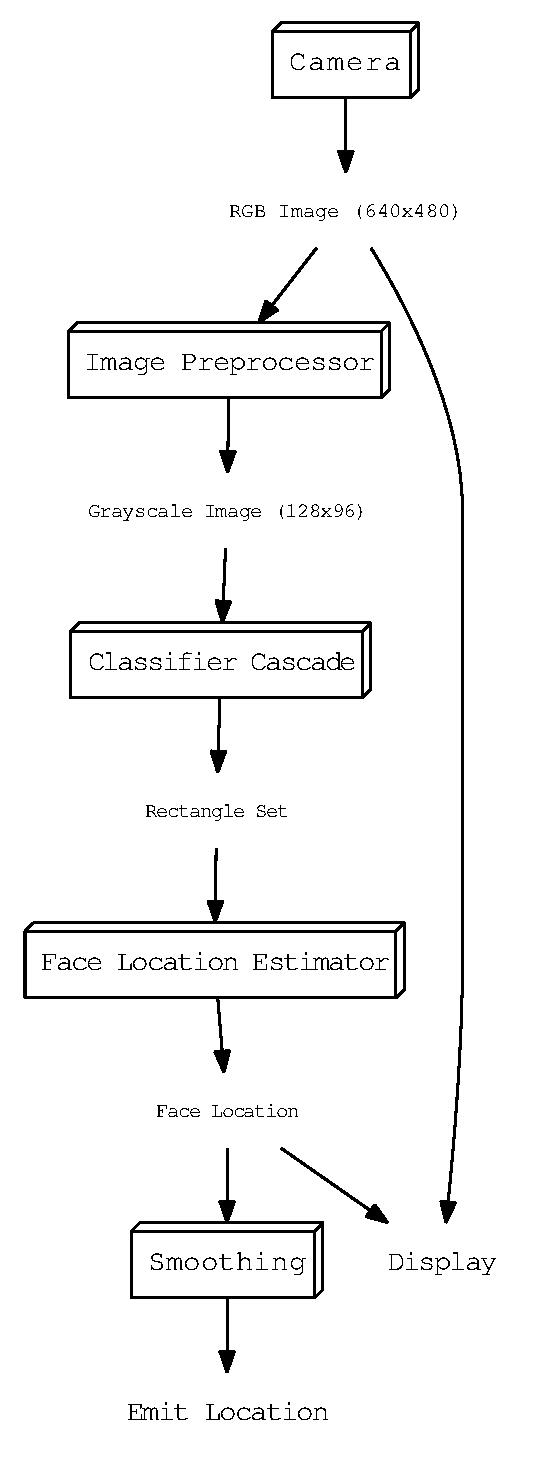
\includegraphics[scale=0.6]{figures/facearch}
  \caption{Architecture of the face detection subsystem}
  \label{fig:facearch}
\end{figure}

The face detector's architecture is shown in \figref{facearch}. The
system polls the camera for a frame. The frame it receives in return
is a raw image in Ipl format (which is OpenCV native format) which is
in full color and is 640 pixels by 480 pixels. This image is copied
(for display later) and then downsampled by a factor of five and
converted to grayscale. This grayscale 128-by-96 image is then fed
into the Haar classifier cascade. The classifier returns a series of
rectangles which define the estimated bounds of the face. The facial
location estimator finds the centroids and areas of each of these
rectangles. It then examines the normalized difference between the
last decision it made (i.e., where it decided the face was in the last
frame) and all possible decisions for this frame, and takes the
rectangle that minimizes this difference to be the current location of
the face. This is important, as the cascade will often detect faces
where there are none; however, usually these can be culled by just
looking at the relative area of the rectangles, as the false positives
are usually either very large or very small. Once it has found the
probable face location, it emits the location of the face and updates
the live monitor display.

This system is not without its drawbacks. I noticed that it was mildly
sensitive to lighting conditions, although it only becomes a real
issue in degenerate lighting conditions where the user is backlit and
therefore in silhouette. It also, interestingly enough, was sensitive
to my glasses. I have heavily-framed glasses, and occasionally it
would lose track on my face with my glasses on. This was especially
true when the lighting was less than optimal; when lighting was good,
the glasses didn't seem to make much of a difference. When lighting
was poor, though, taking off my glasses would often result in a
perfect track where tracking with glasses on was spotty at best.

\subsubsection{Smoothing Methods}
While the classifier method resulted in fairly stable detection, there
was still noise in the detection results. I got around this by using a
standard smoothing algorithm called exponential smoothing. It treats
the output of the face estimator as a linear recurrence, and defines a
second first-order linear recurrence in terms of the previous smoothed
value and current face value. The exact recurrence is as follows

\begin{align*}
  s_1 &= x_0 \\
  s_{t+1} &= (1 - \alpha) x_t + \alpha s_t, \; t \ge 1
\end{align*}

Where $s_n$ is the nth smoothed face value, $x_n$ is the nth detected
face value, and $\alpha$ is a smoothing factor. Higher values of
$\alpha$ mean that the system responds to movement slower, but the
output is smoother, while low $\alpha$ means low latency but higher
jitter. I found that I wanted different smoothing values on the
different axes, because the classifier was better at detecting along
certain axes. More specifically, it did an better job of reliably
determining the face's location along the image's y-axis, but a very
poor job of estimating the size of the face (which I used to determine
the z-component of the face's location). In the end, I used $\alpha_x
= 0.65, \; \alpha_y = 0.6, \; \alpha_z = 0.8$, which resulted in a
fairly accurate and low-latency response to movement, with very little
jitter.

